\documentclass{sig-alternate}
\usepackage{subfigure, graphicx, url}

\newcommand{\strong}[1] {\textbf{#1}}
\newcommand{\code}[1] {\texttt{#1}}

\begin{document}
\title{Text Sliding: Information Discovery with Intensely Integrated Text Analysis}
\numberofauthors{4}

\author{% 1st. author
\alignauthor Firstname LastName\\
       \affaddr{Address}\\
       \affaddr{Address}\\
       \affaddr{Address}\\
       \email{email@address.edu}
% 2nd. author
\alignauthor Firstname LastName\\
       \affaddr{Address}\\
       \affaddr{Address}\\
       \affaddr{Address}\\
       \email{email@address.edu}
% 3rd. author
\alignauthor Firstname LastName\\
       \affaddr{Address}\\
       \affaddr{Address}\\
       \affaddr{Address}\\
       \email{email@address.edu}
}

\maketitle

\begin{abstract}
There are numerous information analysis and discovery tools that allow users to view multidimensional data from different angles by selecting subsets of data, viewing those as visualizations, moving laterally to view other subsets of data, slicing into another view, expanding the viewed data by relaxing constraints, and so on.  However, these tools operate over numerical and categorical data, but do not seamlessly operate over raw textual information with the same flexibility. In this paper we describe a text analysis and discovery tool that allows for highly flexible  ``slicing and dicing'' (hence  ``sliding'') across a text collection.  The goal of the tool is to help scholars and analysts discover patterns and formulate and test hypotheses about the contents of their text collections, midway between what traditional humanities scholars call a  ``close read'' and the digital humanities  ``distant read'' or "culturomics" approach.  We illustrate the text sliding capabilities of the tool with two real-world case studies from the humanities and social sciences -- the practice of literacy education, and U.S. perceptions of China and Japan over the last 30 years -- showing how the tool has enabled scholars with no technical background to make new, important discoveries in these text collections.

\end{abstract}

% A category with the (minimum) three required fields
\category{H.X}{XXXXX XXXXXXX XXXX}{XXXXX}

%A category including the fourth, optional field follows...
\category{H.X}{XXXXX }{XXXXX }[XXXXX ]

\keywords{exploratory data analysis, text mining, information visualization, digital humanities}

\section{Introduction}
Current text analysis systems put computational linguistics and data visualization into the hands of users. Tools such as Jigsaw, IBM TextMiner, and SAS Text Analytics take techniques like text classification, named-entity recognition, sentiment analysis and summarization and build systems to automate their use. To make the results of these computational analyses interpretable, they display the outputs with interactive data visualization. These systems have made advanced text mining and visualization algorithms available to users without expertise in those areas.

However, language is a unique form of expression, and text as data is distinct from numerical and categorical data.  Text has both linear and hierarchical structure, its meaning is ambiguous given its representation, it has tens of thousands or hundreds of thousands of features, and frequencies of words are distributed via a power law.  

Even a small fragment of text does not stand alone, but is densely interconnected with other text through the \emph{linguistic phenomena} that it contains. These are units of meaning that take surface form in text, such as words, phrases, relations between words (including synonymy and hyponymy) and literary devices, such as metaphor, sarcasm and allusion. To illustrate, consider this 13-word ``slice'' of text from Shakespeare's ``Romeo and Juliet", where a slice is simply a set of sentences (not necessarily consecutive, like in this example):

\begin{verbatim}
ROMEO:
    Is she a Capulet?
    O dear account! my life is my foe's debt.
\end{verbatim}

Surrounding this tiny slice is a swarm of other slices of text, each associated with the different linguistic phenomena in this slice. For instance:
\begin{itemize}
\item Each of the 11 distinct words in the above excerpt can be thought of as a jumping-off point to all of the other sentences in which it occurs, as well as to sentences containing other words that mean the same thing, or to other words that tend to be used near it.
\item Each  two-, three-, or n-word phrase can be associated with every other sentence in which it occurs.
\item  Each grammatical relationship between words (such as ``dear" being an adjective modifier of  ``account") can be thought of as a link to other words that enter that relation (other adjectives describing ``account", or other things that are ``dear").
\item Each instance of a literary device, such as the exclamation ``dear account'', or the imagery of debt, can be associated with all other occurrences of this phrase, or the different phrasings with which this concept surfaces in the play.
\end{itemize}

The more structure there is to text, the more kinds of associations are possible. Shakespeare plays have metadata, such as speaker, act, and scene, so associations based on these dimensions also exist:
\begin{itemize}
\item The speaker, Romeo, can be associated with all the other speeches by him.
\item The location within the play: Act 1, Scene 4 can be associated with the other scenes in that act, or the all speakers in that scene.
\end{itemize}

This network of associated slices is apparent to the reader. And to an analyst trying to make sense of an idea, some associations may be deeply meaningful.  Transitions  and associations are central to the text analysis process, and people seeking knowledge from text are engaging in \emph{sensemaking}. They do not follow a straight path from data input to analysis output, but meander between analysis, interpretation, exploration and understanding on different sub-collections of data.  It is therefore important for text analysis systems to support not just algorithmic and visual analysis, but the transitions: slicing, filtering and exploration that lead from analysis to analysis, visualization to visualization, and finally to insight.

In this paper, we describe a text analysis tool called WordSeer that supports such transitions.\footnote{This is version 3.0 of WordSeer, which has notably more flexible interactions than older versions.}  It allows highly flexible slicing and dicing, as well as frictionless transitions (hence ``sliding") between visual analyses, drill-downs, lateral explorations and overviews of slices in a text collection. Our tool uses computational linguistics, information retrieval and data visualization, and enables scholars with no technical background to conduct analyses yielding concrete, useful and otherwise inaccessible knowledge. 

This paper is structured as follows: in the next section, we describe our motivating field of humanities and social sciences and the theory of sensemaking that motivates the need for ``sliding'' interactions between slices. After that, we explain the main ideas behind text sliding and show it in action with extended examples from case studies. Then, we describe related systems, and finally conclude with a discussion our results and future work.


\section{Motivation}

\subsection{Humanities and Social Sciences}
The design of the tool is motivated by the desire to support the humanities and social sciences (HASS). In these fields, it is common for scholars to have hundreds, even thousands of text-based source documents of interest from which they extract evidence for complex arguments about society and culture. These collections (such as the set of all New York Times editorials about China, the complete works of Shakespeare, or the set of all 18th Century American novels)  are difficult to make sense of and navigate. Unlike numerical data, they cannot be condensed, overviewed, and summarized in an automated fashion without losing significant information. And the metadata that accompanies the documents -- often from library records -- does not capture the varied content of the of the text within.

HASS scholars are an important area of focus for tool builders for another reason: low uptake. A 2012 study of computational tool use among these scholars showed that adoption was low despite an abundance of tools. The main culprit? Poor interface design. In our research, we have tried to avoid this problem by taking an iterative, user-centered design approach. We collaborate with active HASS scholars working on text analysis problems of existing professional interest to them, and let their needs, behaviors, and observations drive tool development.

We introduce the text sliding capabilities of WordSeer using two case studies. The researchers driving these studies successfully used the tool to further their projects. The two projects investigated:
\begin{enumerate}
	\item How college students from diverse backgrounds remember and reflect upon literacy.
	\item How U.S. perceptions of China and Japan responded to China's rise over the last 30 years.
\end{enumerate}


\subsection{Supporting Sensemaking}

Observational studies from the literature on sensemaking describe many problems analysts encounter while trying to make sense of text collections. These studies typically study professionals such as government intelligence analysts \cite{x}, business analysts \cite{x} market researchers \cite{x} and academics \cite{x} at work, attempt to categorize the actions they perform and identify common sequences of actions. Several models of the sensemaking process have emerged \cite{x} These models attempt to explain what one would observe when watching analysts distill "understanding" from raw data, where understanding usually manifests itself as a summary, report, or presentation.

Pirolli and Card \cite{pirolli_sensemaking_2005} identified ``pain points" in three areas having to do with navigation and transitions between slices while studying intelligence analysts working with large collections of text-based reports:
\begin{enumerate}
\item \strong{Exploring} the collection by searching and filtering. Collections were often difficult to navigate. 
	\begin{itemize}
		\item Design Goal: make associated slices were easy to see and to access, so exploration  becomes easier. 
	\end{itemize}
\item \strong{Enriching}, which is the process of collecting a narrower set of items for analysis. This is a time consuming process involving going through documents returned by results, reading them to determine whether they were relevant or not, and placing them into groups.
	\begin{itemize}
		\item Design Goal: Make it easy to select documents matching a term, quickly skim the text to determine relevance, and to collect the relevant text into a slice for later analysis.
	\end{itemize}
\item \strong{Exploiting}, which is the process of analyzing the collected information by manual schematizing, computational analysis, or visualization. Follow-up actions, such as drilling down to a finer set, noticing something interesting and starting a different analysis, or re-framing the question has a high cost.
	\begin{itemize}
		\item Design Goal: make it easy to explore associations and to start new threads of inquiry with low overhead,  without losing current state.
	\end{itemize}
\end{enumerate}




\section{Text Sliding}


\begin{figure}[ht!]
\begin{center}
%
        \subfigure[A single view showing a visualization accompanied by some summary/filters.            \label{fig:intro01}]{%
	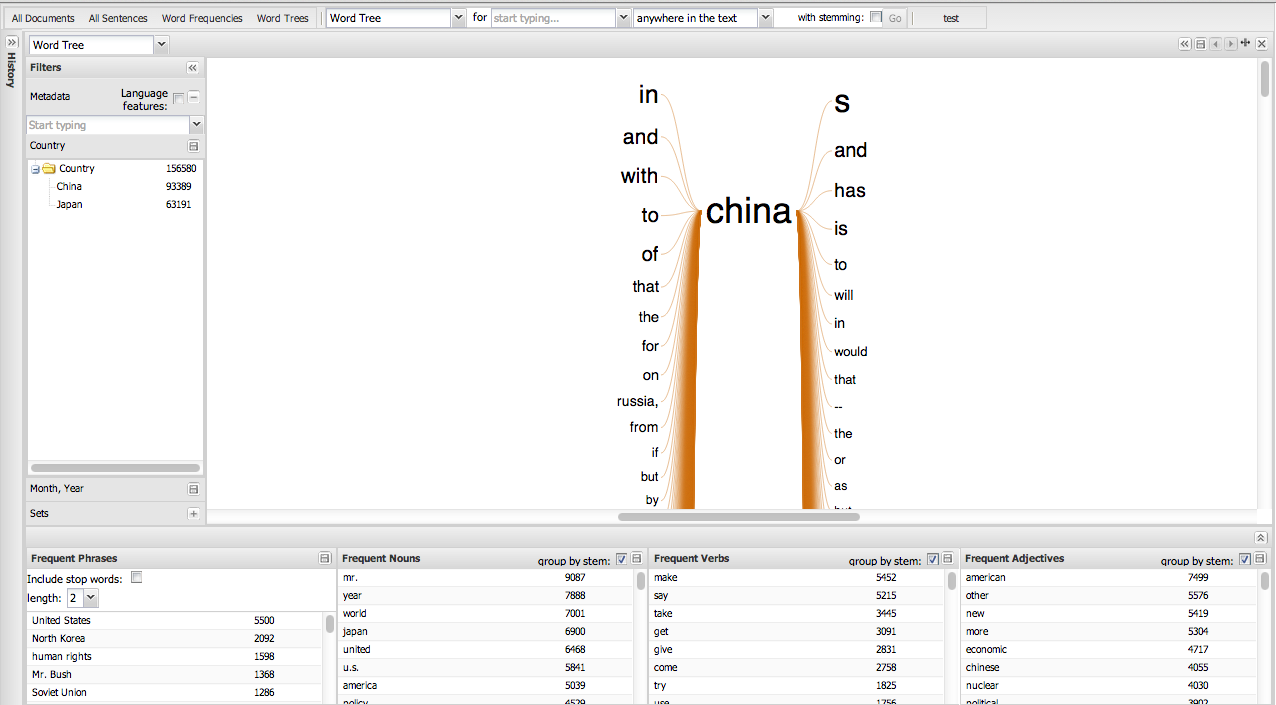
\includegraphics[width=0.5\textwidth]{fig/intro/01.png}
        }%
        \\
        \subfigure[A breakdown of the components of the user interface  \label{fig:intro02}]{%
	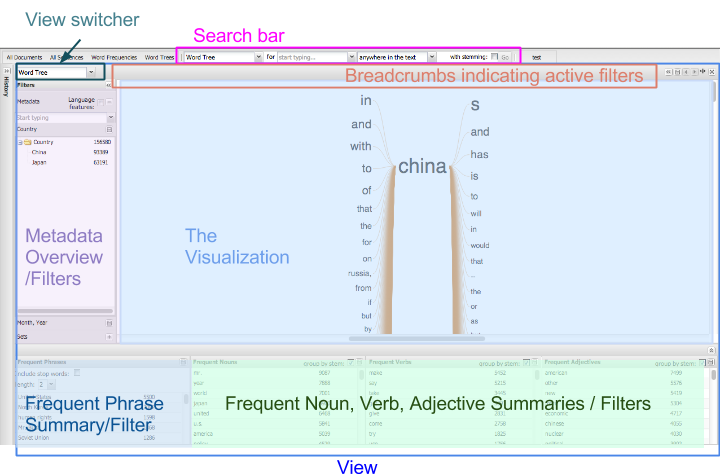
\includegraphics[width=0.5\textwidth]{fig/intro/02.png}
        }%
%
    \end{center}
    \caption{%
        What C.F. sees when he opens up his editorials in WordSeer.
     }%
\end{figure}

When a user opens up WordSeer for the first time, rather than showing a blank screen a requiring the user to think up a query, the tool  provides summary statistics immediately, as shown in Figure \ref{fig:intro01} on a collection of \emph{New York Times} editorials.  Figure \ref{fig:intro02} breaks this down into its core components. This is a single \emph{view} with a \emph{Word Tree} visualization of the most frequent content word in the \emph{slice} ``the entire collection''. 

Word Trees \cite{wattenberg_word_2008} are interactive visualizations that allow a user to explore the contexts in which a word is used. They group together common left- and right-contexts into a tree that gets finer and finer as the context get longer, terminating in individual sentences.  Because no query has yet been specified, the Word Tree view centers on the most frequent content word in the collection (content words exclude very common (stop) words, such as ``the'', ``a'', ``and'', etc.). In this case, the most frequent content word is ``China'' (see first case study below).  Other visualizations are also available, including a tabular list of sentences along with their metadata, a heatmap showing the location of query terms within each document, and bar charts and other statistics about the distribution of the metadata and the query terms, as described below.

The paired concepts of \emph{slices} and \emph{views} are central to text sliding. A slice is a set of sentences, and a view is a visual representation of the data in a slice: the view can range from a simple vertical list of the sentences in the slice, to more complex linguistic processing combined with visual analytics.  A slice is like a scientific specimen or a sample of some chemical compound,  and a view is a lens or a test that reveals different information about the sample.
(Currently we define a slice as \emph{a set of sentences}, although in future it might use different units of text, such as paragraphs, documents, or phrases.) We allow arbitrarily-assembled slices, but it is easiest to think of slices as combinations of searches and filters.  


Text sliding is a way to move from a view of a slice to a different view. Through the richness of language, slices can be associated with many other slices (such as those that contain the same  words, phrases, or ideas). If there is metadata accompanying the text, such as year, and topic, as in these editorials, the user can take advantage of these  \emph{metadata associations}.  Finally, through the wide variety of visual analytics tool available, there are several different ways of viewing and analyzing the data in a single slice. Text sliding makes all these associations accessible in a ``low friction" way.

In detail, we define text sliding as:
\begin{itemize}
	\item Getting a different view of the same slice, or
	\item Opening a new view of an associated slice, which can consist of
	\begin{itemize}
	  \item drilling down (narrowing, selecting), or
	  \item following a new thread (moving laterally) or
	  \item finding related words or sentences  (also moving laterally)
	 \end{itemize}
\end{itemize}

\subsection{Views}
Views  are window-like panels, and the user can open up any number of panels in the interface to facilitate comparison across views.  Views contain the following components, as illustrated in Figure \ref{fig:intro02}:
\begin{itemize}
	\item A drop-down menu for switching to a different view of the same slice (see Figure \ref{fig:chris03}),
	\item Breadcrumbs describing the searches and filters that define the current slice,
	\item A visualization of the data in the slice. Currently, the choices are:
		\begin{itemize}
			\item A list of sentences,
			\item A list of documents that match the sentences in the slice,
			\item An interactive Word Tree \cite{wattenberg_word_2008} of the most common word in the slice, or the search term, if specified,
			\item Charts showing distributions of the slice's sentence counts across various metadata categories,
			\item A document reader,
			\item Bar charts showing how often different words in the slice  appear in grammatical relations.
		\end{itemize}
	\item Summary statistics of:
		\begin{itemize}
			\item How many sentences within the slice match different metadata categories,
			\item The most frequent nouns, verbs, adjectives and multi-word phrases in the slice.
		\end{itemize}
\end{itemize}

The simplest sliding interaction in WordSeer is creating a different view of the same slice.  There is a drop-down menu at the top left corner of each view which provides this function (Figure \ref{fig:chris03}).  Selecting a different view from the menu opens up that new view (on the same slice) alongside the current one. Users can have as many views open as they want, but most displays get crowded after two are three are open; the tool allows the panels to be collapsed and a history panel allows revisiting of earlier views.  
\begin{figure}[h!]
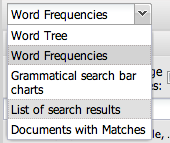
\includegraphics[width=0.2\textwidth]{fig/chris/03.png}
\caption{ The view-switcher drop-down menu, found at the top left corner of every view. Selecting an option opens a new view  of the same slice alongside the current view. \label{fig:chris03}}
\end{figure}

\subsection{Slices}

The primary way in which WordSeer allows users to make slices is by intersecting \emph{searches} and \emph{filters}.  A search restricts the collection to just the sentences matching the query, and a filter restricts it to just sentences matching a particular metadata value. 

Case study 1 (see below) illustrates the importance of allowing users to compose their own slices from the contents of a  broader collection. In the study, the scholar `C.F.', an English PhD candidate whose dissertation focuses on how US literature responded to the rise of China, used a collection of  the last 30 years of \emph{New York Times} editorials about China and Japan to get a sense of how perceptions towards those countries have shifted.

His first goal was to get a sense of the differences in the way China was discussed in the 80's, 90's and 00's. To do this, he assembled three slices by starting with a \emph{search} for ``China'' (Figure \ref{fig:intro03})  and then filtering the `Year' category to range over a decade (Figure \ref{fig:intro04a}).  WordSeer also allows filtering by categorical values. If he had wanted to, he could have filtered these results to just editorials whose main topic was China or Japan, using the controls shown in Figure \ref{fig:intro04b}. 
\begin{figure}[ht!]
\begin{center}
	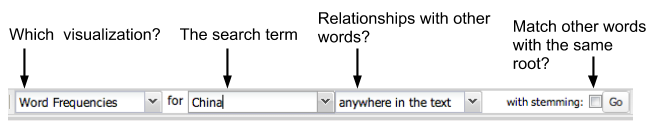
\includegraphics[width=0.5\textwidth]{fig/intro/03b.png}
\end{center}
    \caption{%
        Creating a slice by searching for the word ``China''. This creates a slice containing only sentences that contain the word ``China''. \label{fig:intro03}
     }%
\end{figure}

\begin{figure}[ht!]
\begin{center}
%
        \subfigure[C.F. used the numerical/date ranges from the Metadata Filter  to filter the slice ``all sentences containing \emph{China}" to sentences from the 90's. ]{%
            \label{fig:intro04a}
	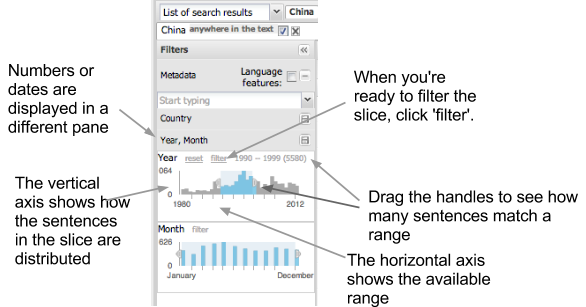
\includegraphics[width=0.5\textwidth]{fig/intro/04b.png}
        }%
        \\
         \subfigure[How to use the categorical metadata overview to filter the slice ``all sentences containing \emph{China}" to only sentences from editorials about China.]{%
            \label{fig:intro04b}
	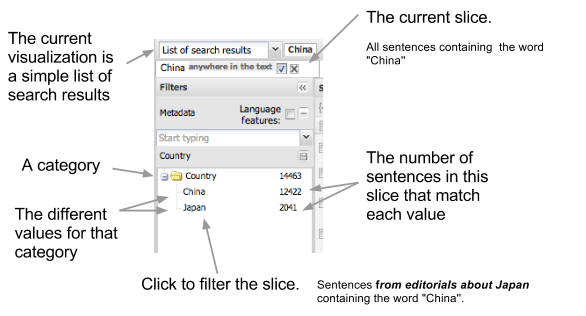
\includegraphics[width=0.5\textwidth]{fig/intro/04a.png}
        }%
%
    \end{center}
    \caption{%
     Overviews double as filters, which can be used to create or narrow down a slice \label{fig:intro04}.
     }%
\end{figure}

\subsection{Grammatical Relations}

 In our database, each sentence is indexed according to the following linguistic phenomena:
\begin{itemize}
  \item Each word in the sentence, and its part of speech (noun, verb, adjective, etc.)
  \item Each consecutive two-, three-, and four-word sequence in the sentence
  \item Each grammatical relationship in the sentence. (These are identified using a dependency parser  explained in \cite{jurafsky_chapter_2009}. In particular, we use the Stanford dependency parser\cite{klein_accurate_2003}).  The parser extracts many kinds of relationships, but some of the more easily understood ones include \emph{noun compound}, where two nouns come together to signify a new concept, \emph{adjective modifier} where an adjective describes another word, and \emph{direct subject} in which a word is the agent of a verb.
  
\end{itemize}
By traversing these indexes, we can quickly compute the associations for a slice. From a slice, we can query for all the words, phrases, or grammatical relations in the sentences in that slice, and from there, to all the other sentences that contain each particular item.  


Each view automatically presents the most common nouns, verbs, and adjectives (Figure \ref{fig:intro06}), as well as the most common phrases (Figure \ref{fig:intro07}), along with their counts, in a panel at the bottom.    
\begin{figure}[ht!]
\begin{center}
	
\includegraphics[width=0.5\textwidth]{fig/intro/06a.png}
	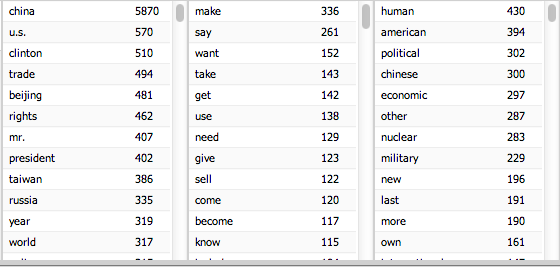
\includegraphics[width=0.5\textwidth]{fig/intro/06.png}
\end{center}
    \caption{%
        Each view automatically shows the most frequent nouns, verbs, and adjectives in the slice, along with their counts, in a bottom panel. This is a zoomed-in view of the bottom panel of Figure 1 \ref{fig:intro01}, which shows the most frequent words in the \emph{New York Times} editorals for case study 1 below.  \label{fig:intro06}
     }%
\end{figure}

\begin{figure}[ht!]
\begin{center}
	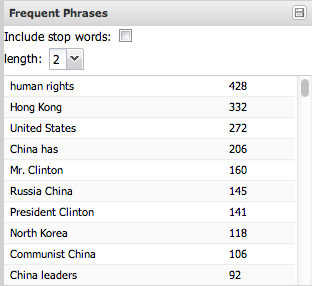
\includegraphics[width=0.2\textwidth]{fig/intro/07.png}
\end{center}
    \caption{%
        A zoomed-in view of the bottom panel of Figure 1 \ref{fig:intro01} showing the most frequent phrases in the \emph{New York Times} editorals for case study 1 below.  \label{fig:intro07}
     }%
\end{figure}

Individual words are jumping-off points. They can be acted upon wherever they appear via the Word Menu (Figure \ref{fig:intro08}). The word menu is how WordSeer enables \emph{lateral movement}.  Any time a user sees a word, they can follow up on it by examining the grammatical relations in which it occurs, seeing related words,  and creating visualizations of the slice of sentences that contains the word, as well as the slices containing various relationships to other words.

\begin{figure}[ht!]
\begin{center}
	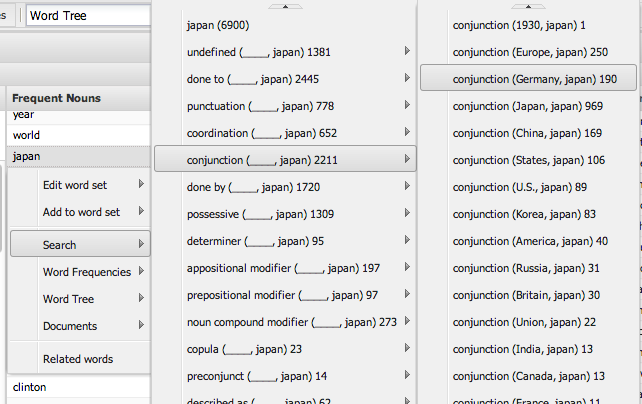
\includegraphics[width=0.5\textwidth]{fig/intro/08.png}
\end{center}
    \caption{%
      The Word Menu for `japan'.  The search options show how often `Japan' appears in different grammatical relations. Expanding upon the `conjunction' relation, for example, shows that `Japan' appears in the  `conjunction' relation  2211 times, and is most often paired with Europe, Germany, the US, Korea, Russia, and Britain. Clicking on any of the menu options opens up the slice of matching sentences in a new view \label{fig:intro08}}%
\end{figure}


\begin{figure}[ht!]
\begin{center}
	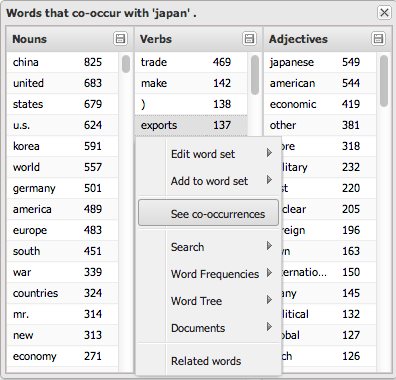
\includegraphics[width=0.5\textwidth]{fig/intro/09.png}
\end{center}
    \caption{%
 		The nouns, verbs, and adjectives that co-occur most frequently with `Japan'. Clicking on any of these words opens up a Word Menu, this time with the option to see co-occurrences.  Clicking on the option  above opens up a view of the sentences in which `Japan' and `exports'  co-occur.
	\label{fig:intro09}}%
\end{figure}


The related words option in the Word Menu shows the nouns, verbs, and adjectives that co-occur most frequently with the clicked-on word. For example, if we click on `Japan' and open up the related words (Figure \ref{fig:intro09}) the pop-up shows the words that co-occur most frequently with `Japan'. Each of these related words words can be clicked in turn, opening up a new Word Menu. These menus have the additional option to `See co-occurences', as shown in the new Word Menu for `exports'. That option opens up a new view showing just those sentences in which the two words appear together  (in this case, `Japan' and `exports'). 

The word menu reduces friction in both discovery and search. It only takes one menu click to discover that `exports' occurs frequently with `Japan', and only one more to see all the sentences in which `Japan' and `exports' are mentioned together.  


\subsection{Custom Slices with Sets}

Searches and filters are useful, but cannot always express  specific analysis goals. WordSeer therefore allows users to construct custom slices through Word-, Sentence-, and Document Sets. These custom slices behave like any other slices, which means that they can be summarized in views,  analyzed, filtered and searched. But they are more powerful that other slices because they also behave like metadata, making them \emph{categorical filters}.

Word Sets are perfectly illustrated by an example from Case Study 1 (see below). One concept of interest in this study was ``growth''. The scholar wished to investigate the occurrence of growth-related words in editorials about China.  

First, he needs to create a new word set and type in some growth-related words (Figure \ref{fig:intro10a-word-sets}). The result is a Word Set representing a new slice of sentences, those containing at least one of those words. 

\begin{figure}[ht!]
\begin{center}
%
        \subfigure[Creating a ``growth'' word set with 6 words in it. \label{fig:intro10a-word-sets}]{%
	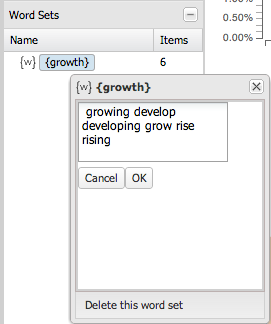
\includegraphics[width=0.2\textwidth]{fig/intro/10a-word-sets.png}
        }%
        \\
        \subfigure[The set now appears in the drop-down menu in the search box. \label{fig:intro10b-word-sets}]{%
	
\includegraphics[width=0.5\textwidth]{fig/intro/10b-word-sets.png}
        }%
         \\
        \subfigure[The set also appears in the word menu  \label{fig:intro10c-word-sets}]{%
	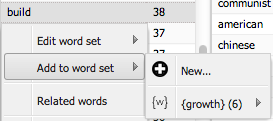
\includegraphics[width=0.2\textwidth]{fig/intro/10c-word-sets.png}
        }%
        \quad
        \subfigure[ The set also appears in the metadata overview   \label{fig:intro10d-word-sets}]{%
	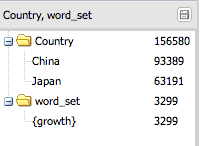
\includegraphics[width=0.2\textwidth]{fig/intro/10d-word-sets.png}
        }%
%
    \end{center}
    \caption{%
       Word Sets in WordSeer. \label{fig:intro10-word-sets}
     }%
\end{figure}
Once the word set is created, the entire user interface responds to its presence. The search box now shows a drop-down option for the set  (Figure \ref{fig:intro10b-word-sets}).  The word menu shows the option to add a new words (Figure \ref{fig:intro10d-word-sets}) and the metadata overviews (Figure \ref{fig:intro10d-word-sets}), previously restricted to pre-defined categories,  now show this new ``category'', and allows him to filter based on it.   

\begin{figure}[ht!]
\begin{center}
	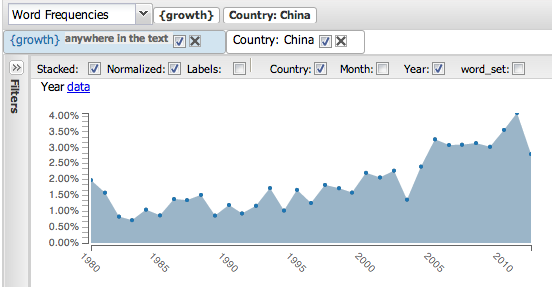
\includegraphics[width=0.5\textwidth]{fig/chris/04a.png}
\end{center}
    \caption{%
	A Word Frequencies view of the slice corresponding to the \code{\{growth\}} word set shows that the frequency of this group of words in \emph{New York Times} editorials about China steadily increases between the 1980s and 2000s. \label{fig:chris04a}
     }%
\end{figure}

Finally, he selects the  \code{\{growth\}} Word Set as his search query, opens a Word Frequencies view, and applies the \code{ country = China} filter to focus on editorials about China. The resulting visualization is Figure \ref{fig:chris04a}, which shows almost a doubling of the frequency of these words over the 30-year period from 1980 to 2012.

For sentences and documents, the idea is the same.  Users can hand-pick collections of sentences from the reading view, and from search results view, or collections of documents from the document search results view.  Once created, all these sets can be overviewed and analyzed like any other slice, and additionally used as filters.

\section{Case Study: U.S. Perceptions of\\China Japan}

C.F. is a PhD student at [university's] English department. His dissentation explores how US literature has responded to the rise of China since it began liberalizing its economy in the late 1970s.  His arguments depend upon a set of historical observations about the rise of China  broadly accepted by historians and cultural historians: 
\begin{enumerate}
\item From the 1970s prior to the Tiananmen Square crackdown in 1989, US observers paid more attention to Japan than China. During this period, China did not have  more than a strategic, Cold War relevance. 
\item With the onset of the 1990s, attention shifts from Japan to China. Japan entered its first ``Lost Decade'' of economic stagnation, and China, meanwhile, began deepening its economic relations with the US.
\item After China's accession to the World Trade Organization in 2001, US-China bilateral relationship becomes increasingly important to global economics and politics.
\item After 2001, there is an increasing sense that the US's time as the post-socialist era's last remaining superpower are numbered, and that China will replace it.
\end{enumerate}
Literary scholars typically allow their claims to rest on observations made by field experts like historians and sociologists, or on their own inductive reasoning. C.F., however, sought to supply these observations with as much empirical evidence as possible, as well as to verify them.

To generate this evidence, C.F. collected \emph{New York Times} editorials from  the Lexis/Nexis database, from 1980 to 2012. Using Lexis/Nexis's metadata, C.F. limited the corpus to those tagged with subjects ``China" or ``Japan." This resulted in a set of 5,715 editorials which were then imported to the tool.

After a few weeks of face-to-face meetings in which we discussed his research goals and demonstrated how to use WordSeer to ask questions, C.F. gradually became comfortable using WordSeer on his own. After that, we continued to meet, but focused on discussing his progress, and to on plans for new analysis features based on his needs.

By the end of his project, C.F. had used WordSeer to find evidence for all four observations above. In this paper, we elaborate on numbers 1 and 3, because those investigations made are particularly heavy use of text sliding.


\subsection{Confirming Intuitions}
After becoming comfortable with WordSeer's functionality, C.F's first goal was to get a sense of the tone towards China in the three different decades in his collection: the `80s, `90s, and `00s.  He already had some intuitions of what he would find, but never having used the \emph{New York Times} editorials, or done any previous computational analysis, he wanted to test both the reliability of his corpus, and the ability of WordSeer to replicate well-known facts.

Using a combination of filters for the different year spans and a search for ``China'', C.F. assembled three different slices of sentences mentioning China, one for each decade. Then, he opened up each decade in a different view and compared the most frequent words and phrases (from the automatically-generated overviews).

\begin{figure}[h!]
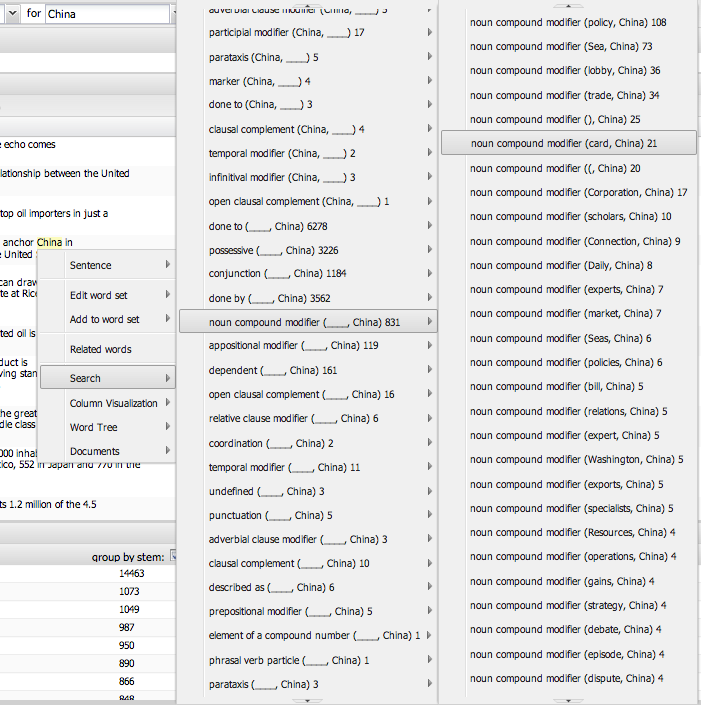
\includegraphics[width=0.5\textwidth]{fig/chris/01.png}
\caption{The word menu for China allows a user to explore all the grammatical relationships in which ``China'' participates.   After selecting \emph{China > Search > noun compound modifier}, the noun-compound relationship ``China card'' stood out to C.F. \label{fig:chris01}}
\end{figure}

Fortunately, WordSeer's overviews showed clear differences between the decades. Each part of speech revealed a different trend in China's changing relationship with the US. 
For instance, the increasing  frequencies of certain growth-related verbs contributed to a sense of China's rise.
\begin{itemize}
\item ``grow, growing'':  294, 232, 421
\item ``rise, rising'': 101, 134, 249
\item ``develop, developing'': 274, 404, 476
\end{itemize}
Using the Word Frequencies visualization in combination with Word Sets, he was able to get a clearer picture. First, he grouped these six verbs into a ``growth'' word set, and then visualized its frequency over time in the China editorials (Figure \ref{fig:chris-growth-over-time}).  The result is a graph showing a steady increase, almost a doubling, of growth-related words in editorials about China.

This first investigation allowed C.F. to rest easy. Secure in having re-discovered the rise of China, he returned to his original questions.

\subsection{1980's: Insignificant, Except for Cold War Strategy}
While comparing the most frequent adjectives for the three decades C.F noticed a drop-off in cold war words. ``Soviet''  went from 1029 in the 1980s to only 80 in the 2000s, and ``communist'' went from 284 to 112.   To investigate the drop-off in more detail, he used the the Word Menu to quickly open up word frequency plots for these two words over time, and filtered them to just the editorials about China.  Figure \ref{fig:chris04b} shows a plot of these words together:

\begin{figure}[h!]
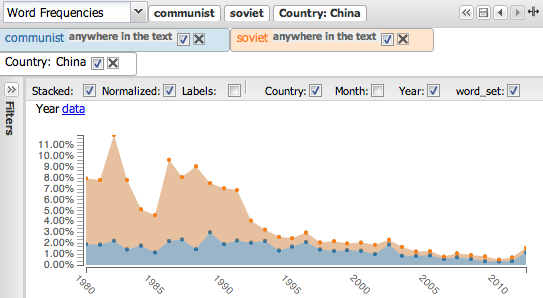
\includegraphics[width=0.5\textwidth]{fig/chris/04b.png}
\caption{The Word Frequencies of `communist' (blue) and `soviet' (orange) in the editorials about China over time. In the early `90's almost 1 in 10 sentences about China mentions one of these two terms. However, in the early `90s, there is a sharp decline, and the terms gradually decrease in frequency over the remaining 20 years. \label{fig:chris04b}}.
\end{figure}

Plotting the terms together (Figure \ref{fig:chris04b}) added depth to his initial observation of their decline.  It shows the dominance and equally dramatic drop-off in cold war mentions over this time period. In the early `80s, almost 11\% -- more than 1 in 10 sentences in those editorials -- mentions one of these the cold war terms. By the `90s, however, this association is down to a trickle. 

\begin{figure}[h!]
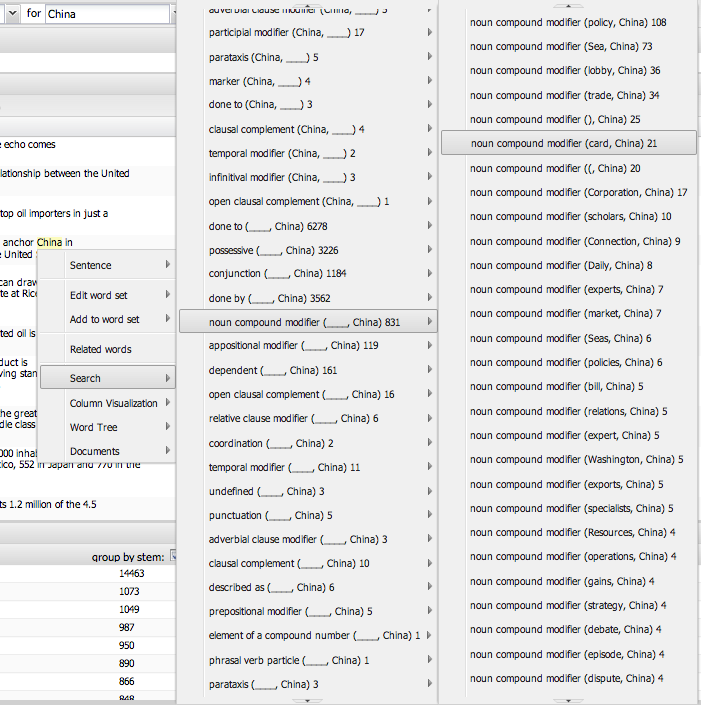
\includegraphics[width=0.5\textwidth]{fig/chris/01.png}
\caption{The word menu for China allows a user to explore all the grammatical relationships in which ``China'' participates.   After selecting \emph{China > Search > noun compound modifier}, the noun-compound relationship ``China card'' stood out to C.F. \label{fig:chris01}}
\end{figure}

An exploration of the ``grammatical neighborhood'' around `China'  helped C.F. find yet more evidence for this idea. This time, it was through a distinctive rhetorical device. As Figure \ref{fig:chris01} shows, clicking on the word ``China'' opens up a menu with search options. These options act as quick previews of different grammatically-related slices: they show the frequencies with which ``China'' occurs in different grammatical constructions with different words.  For C.F., the noun compound relationship yielded a surprise. He noticed an odd construction, ``China card,'' which appeared 21 times.

He immediately explored this this distinctive usage by selecting List of Search Results options for that relationship.  This opened up the list of sentences in which the noun compound ``China card'' occurred.  When C.F. read the sentences, an interpretation suggested itself:
\begin{quote}
[Reading] the sentence search results reveals that phrase is used to refer to the China's strategic value in Cold War geopolitics. Of the four post-2000 instances, only one uses the phrase to describe a contemporary political situation; the others use it to describe Cold War politics. Reducing the vastness of China to a disposable ``card,'' indicates a degree of US self-confidence, not to mention condescension, that disappears after 1989.
\end{quote}

The Word Frequencies view of the same data allowed him to make that temporal claim. Using the drop-down menu at the top left of the panel (Figure \ref{fig:chris03}) he opened up the the word frequencies view alongside his list of search results.  Because the ``year'' metadata was attached to each article, this view displayed a graph of how frequent  sentences containing ``China Card'' were over time (Figure \ref{fig:chris02}). 
\begin{figure}[h!]
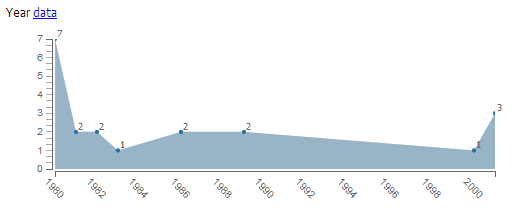
\includegraphics[width=0.5\textwidth]{fig/chris/02.png}
\caption{ The number of sentences matching ``China card'' over time. \label{fig:chris02}}
\end{figure}
The graph shows that ``China card'' the rhetorical figure signifying cold-war strategic value, was used relatively frequently until 1989, but rarely  after that. This confirmed his claim that, up until the early 90's, China had a Cold-war strategic significance to the U.S. that later dissipated.


\subsection{Mid `90's onwards: China's ties with the U.S. Strengthen}
A major event in Chinese international relations occurred in 2001, when china joined the World Trade Organization (WTO).  Although attention had been shifting towards China since the `90s, it is during this period that US-China relations are thought to have become more interdependent, and central to global politics. 

To find evidence for this, C.F.  started with a grammatical structure he thought might make a good proxy for US-China relations: the \emph{conjunction}, which is just an \emph{and} relationship between two words.  He needed a grammatical search because of the possibility of constructions like 
\begin{quote}
``The United States, the world's top energy guzzler, and China, with the world's fastest-growing energy thirst \ldots" (April 2006).
\end{quote}
This fragment places China and the United States in clear conjunction with each other, but an exact-phrase search for \code{`United States and China'} would miss it. 

He created a list of search results view, containing a total of 142 sentences (Figure \ref{fig:chris05}).
\begin{figure}[h!]
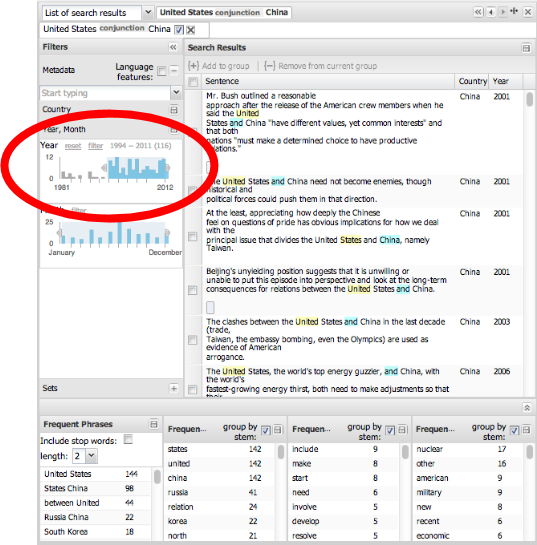
\includegraphics[width=0.5\textwidth]{fig/chris/05-circled.png}
\caption{ The \emph{List of Search Results} view of the slice of sentences matching the  grammatical relationship \code{conjuction(United States, China)}. \label{fig:chris05}}
\end{figure}
A quick look at the distribution of articles over the Year category (circled in red) confirmed his choice of starting point. These were much more frequent from the mid-nieties onward. In fact, out of the 142 occurrences, 116 (81\%) occurred after 1994.

He begain skimming over the results, but soon noticed a problem. While these these sentences did indeed contain many references to US-China relations, they also contained many conjunctions that weren't interesting: purely grammatical ones like ``While maintaining cautious vigilance against rival powers, the United States, Soviet Union, and China separately welcomed this trend.'', and relations involving other parties, like ``In turn, the nuclear five -- the United States, Britain, Russia, France and China -- committed themselves to sign a comprehensive test ban by next year.''

WordSeer's sentence sets are designed to solve exactly this problem. C.F. recognized this, and put them to good use. He manually went through each of the 134 results, and created a sentence set out of the ones that satisfied his criteria: having to do with relations solely between the US and China relations.  He called this set \code{\{US-China relations\}}. Sentences were sometimes ambiguous, but the ease of looking up the sentence within the editorial made it easy to check whether or not it should be included. To quote:
\begin{quote}
[The filtering process] was significantly aided by the ability to click on the sentence and immediately see it located in context within the full editorial.
\end{quote}
He eliminated about half the sentences from consideration, leaving him with a set of  79 sentences. A \emph{Word Frequencies} view of of this smaller slice made the picture much clearer (\ref{fig:chris06}). Of the 79 sentences, the overwhelming majority (86\%) occur after 1995.
\begin{figure}[h!]
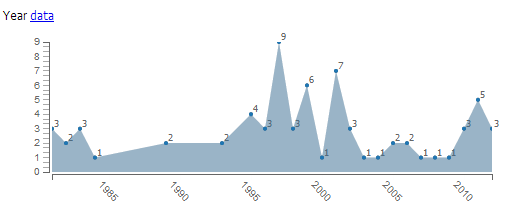
\includegraphics[width=0.5\textwidth]{fig/chris/06.png}
\caption{ The distribution of sentences in in the  \code{\{US-China\} relations slice}.  86\% of the sentences occur after 1994. \label{fig:chris06}}
\end{figure}
C.F. noticed a subtle point: as he moved from the 1990's to the 2000's, the relationship between the US and China seemed to be increasingly  `central' and `inter-dependent':
\begin{quote}
Phrases and words like the following begin to appear: ``21st century's most important relationship,'' ``co-dependent,'' ``interlocking,'' etc. But I achieved a more precise sense of the themes of \emph{interdependence} and \emph{centrality }independence and centrality more precisely using a Word Set of thematically-related adjectives drawn from the Frequent Adjectives overview. Using a the set consisting of ``most central important indispensable dependent interdependent dependency entangled interlocking interdependency'' (taken from the overview). The graph shows that it's not until 1995 that the US-China relationship is characterized by these themes.
\begin{figure}[h!]
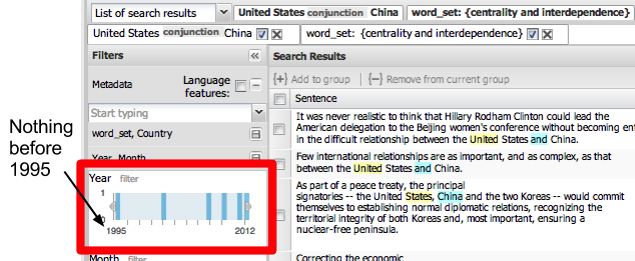
\includegraphics[width=0.5\textwidth]{fig/chris/07.png}
\caption{ The distribution of the \code{\{centrality and interdependence\}} Word Set within the \code{conjunction(United States, China)} slice. There are no occurrences before 1995. \label{fig:chris07}}
\end{figure}
\end{quote}



\section{Case Study: Literacy Autobiographies}

\subsection{Introduction}
As a college English Composition instructor,  R.G., at  [university's] school of Education asks students to write often and in a variety of situations. In this project, he examined ways in which he might draw upon the tool to assist in the teaching and learning of writing. He was particularly interested in the literacy autobiography. In this type of writing, students describe significant experiences they have had with literacy and reflect upon the importance of literacy to their lives.  

R.G. analyzed the content of approximately 140 literacy autobiographies written by students from courses that he has taught over that past two years, each about 1,500 to 2,000 words long. He is familiar with the collection, having previously read and commented on each of the 140 essays included.  Table \ref{table:rex-courses} shows the different courses from which literacy autobiographies were analyzed. The courses were at different colleges and taught at different proficiency levels.

Among the questions that guided his inquiry were the following. In this example, we show how the tool helped him get answers:
\begin{enumerate}
\item What can a distant reading of student literacy autobiographies tell him about students that close readings cannot?
\item What patterns exist in student literacy autobiographies at different course levels and institutions?
\end{enumerate}

\begin{table}
\begin{tabular}{lll}
Course& College & Level \\
\hline
Engl 1A (n=29) & [anonymized] & First-year \\
Engl 201AB (n=28) & [anonymized] & Pre-transfer \\
Engl 5 (n=40) & [anonymized] & Transfer level \\
Edu 140 (n=40) & [anonymized] & Upper division \\
\end{tabular}
\caption{The four different courses, each at a different proficiency level, from which literacy autobiographies were analyzed by R.G. \label{table:rex-courses}}
\end{table}


 \subsection{A new take on students' experiences}

R.G. doesn't usually consider the frequencies of words unless a student repeats one to the point of distraction. However, the tool's very first overview (like the one C.F saw in Figure \ref{fig:intro01}, except on R.G's data) prompted him to consider the significance of individual words and their repeated use.  As he states:
\begin{quote}
From the moment I opened [the tool], `distance' immediately provided new insight and areas of exploration as I was intrigued by unexpected high word frequencies.  The most obvious example is the frequent use of the word ``time" which is not only the most frequent noun but also the most frequent word overall.  As opposed to ``literacy'', ``language'', and any noun or verb forms of ``read'' and ``write'', the Word Tree for ``time'' appears before any term is placed in the keyword search.   I found similar surprises in the adjective and verb frequencies, and these surprises would guide my decision-making and analysis.
\end{quote}

\begin{figure}
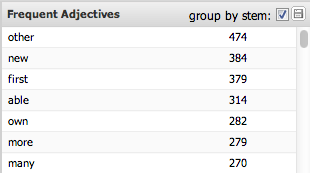
\includegraphics[width=0.5\textwidth]{fig/rex/02.png}
\caption{The most frequent adjectives overall in R.G.'s literacy essays \label{fig:rex02}.}
\end{figure}

Faced with unexpected discoveries in every part of speech, R.G. decided to explore the adjectives (Figure \ref{fig:rex02}). The top three adjectives were not surprising - "other" (474), "first" (379), and "new" (384).  However,  ``able'' (314) and ``own'' (282) were words that he did not expect to be used frequently.

R.G. now wanted to understand the unexpectedly high frequencies of ``able'' and ``own''. WordSeer made this exploration easier. Instead of having to open a new window and type new search queries, clicking on the words themselves opened up Word Menus (Figure \ref{fig:rex03}) which allowed him to create Word Trees centered on those words (Figure \ref{fig:rex04}).   
\begin{figure}[h!]
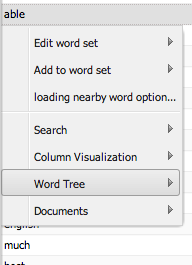
\includegraphics[width=0.2\textwidth]{fig/rex/03.png}
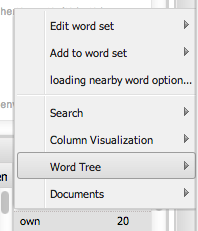
\includegraphics[width=0.2\textwidth]{fig/rex/03b.png}
\caption{Clicking on the ``able" and ``own" in the frequent adjectives list brings up a menu with the option to create Word Trees centered on those words in new panels. The results are shown in Figure \ref{fig:rex04} \label{fig:rex03}.}
\end{figure}

\begin{figure*}[h!]
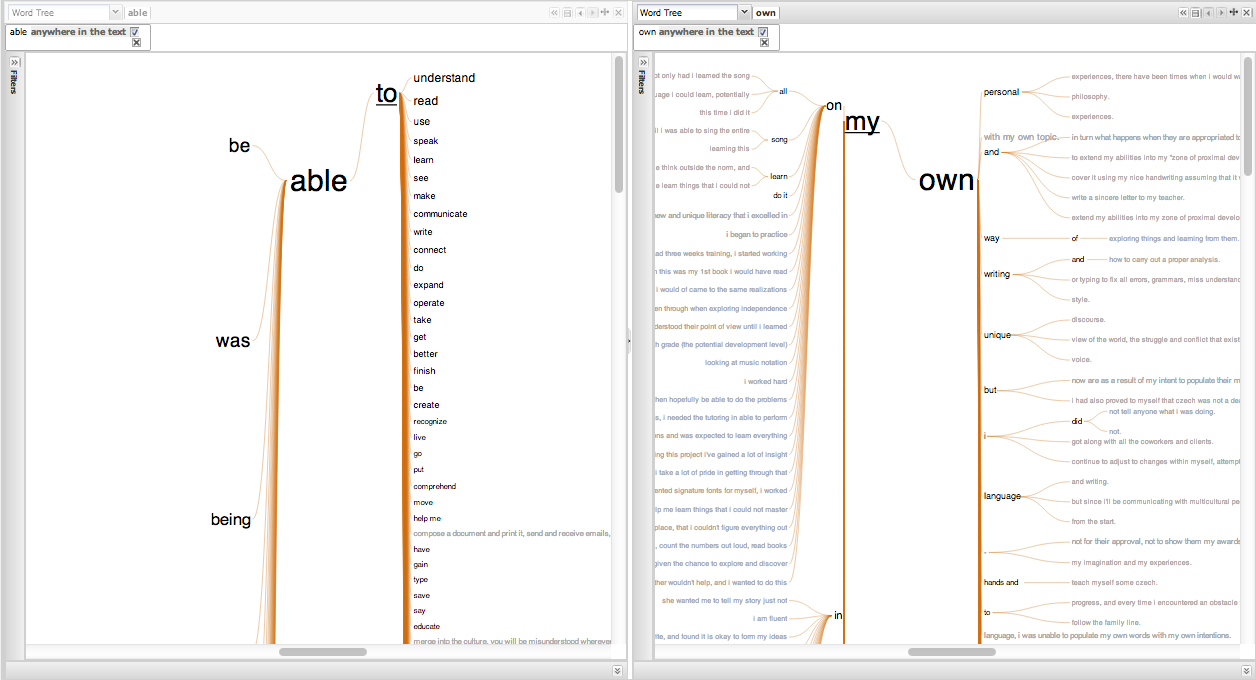
\includegraphics[width=\textwidth]{fig/rex/04.png}
\caption{ On R.G.'s literacy essays data set, two side-by-side Word Trees created from the word menu (with the bottom and side overview panels collapsed). On the left, the tree is centered on `able' and filtered to `able to', and on the right, the tree is centered on  `own' and filtered to `my own' in new panels \label{fig:rex04}.}
\end{figure*}

The Word Tree for ``able" (Figure \ref{fig:rex04} left) revealed that the most common use of the adjective able was: \code{[form of the verb `to be'] + able + to [action verb]}. To get a sense of how common this usage was overall, R.G. hovered over each branch (which displayed the number of sentences under that branch), and adding up the numbers for branches matching ``to be''. He found that the overwhelming majority, 280 out of 314 occurrences, fell into this pattern, with the most common ``abilities'' being literacy-related: read, understand, communicate, learn, speak, etc. For  ``own'' (Figure \ref{fig:rex04} right), the most common construction was: \code{[preposition] + my + own}, with around a third: 100 out of 291 occurrences.  He also used the Word Tree to zoom in and read the individual sentences.

As a result, R.G. came away with a new insight about his students:
\begin{quote}
Student writers articulate their experiences from some first encounter with the unfamiliar, followed by a process of being ``able" to act within that which is becoming less unfamiliar.  Moving into literacy requires these writers to develop their ``own" abilities as necessary to survive and prosper in that context.
\end{quote} 

\subsection{Writing proficiency across courses}
The different courses R.G. taught had different emphases and were taken by students with differing amounts of college education. He was especially interested in differences in sentence construction, hypothesizing that more proficient students would use advanced structures more frequently. To initiate the analyses, he performed word searches on terms such as ``though", ``while", ``although", and ``however", which indicate a complex structure called a ``concessive''. He was expecting consessives to be increasingly frequent as he moved from English 1A, to English 201, to English 5, to Ed140.

The Word Frequencies visualization allowed R.G. to confirm his hypothesis. It shows how often terms occur across different metadata categories (and can shown the counts stacked or grouped, or normalized or raw). R.G. searched for multiple terms simultaneously, which created a comparative visualization (Figure \ref{fig:rex05}).

\begin{figure}[h!]
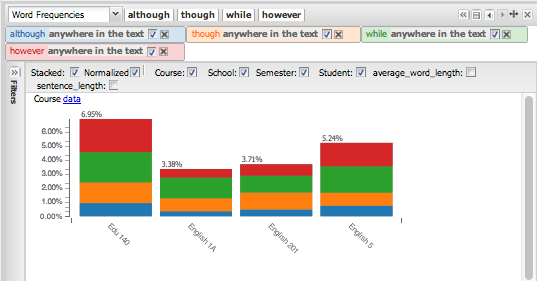
\includegraphics[width=0.5\textwidth]{fig/rex/05.png}
\caption{The normalized frequencies of different "concessive" words. Normalizing the counts adjusts for categories of unequal sizes, showing the percent of matching sentences in different categories instead of the counts. The words are `although' (blue), `though' (orange) `while' (green) and `however' (red). \label{fig:rex05}}
\end{figure}

The increasing frequencies across the course levels confirmed his hunch that as students become more experienced and comfortable with the written word, they used more complex sentence structures more frequently. 






\section

There are numerous information analysis and discovery tools that allow users to view multidimensional data from different angles by selecting subsets of data, viewing those as visualizations, moving laterally to view other subsets of data, slicing into another view, expanding the viewed data by relaxing constraints, and so on.  However, these tools operate over numerical and categorical data, but do not seamlessly operate over raw textual information with the same flexibility. 

Current text analysis systems put computational linguistics and data visualization into the hands of users. Tools such as Jigsaw \cite{}, IBM TextMiner \cite{}, and SAS Text Analytics \cite{} take techniques like text classification, named-entity recognition, sentiment analysis and summarization and build systems to automate their use. To make the results of these computational analyses interpretable, they display the outputs with interactive data visualization. These systems have made advanced text mining and visualization algorithms available to users without expertise in those areas.



Faceted navigation

Subjunctive Interface

WordHoard
Voyeur/Voyage

PaperLens
Tableau

Sandbox/Trist

IBM TextMiner (UIMA)


	



\section{Acknowledgements}
We sincerely thank [Firstname Lastname, Firstname Lastname, and Firstname Lastname] for helpful comments on a Case Study not described in this paper. We are also grateful to [Firstname Lastname] for his helpful advice and thought-provoking discussions throughout.

This work is supported by NEH grant HK-50011-12.

\bibliographystyle{abbrv}
\bibliography{papers} 
  
\end{document}


